%!TEX root = report.tex
\exercise{Principal components}
\subsection{\texttt{IPprincipalcomponents}}
\matlabexternal{../IPprincipalcomponents.m}
\subsection{Reading and arranging images}
\begin{figure}[htb]
 \centering
 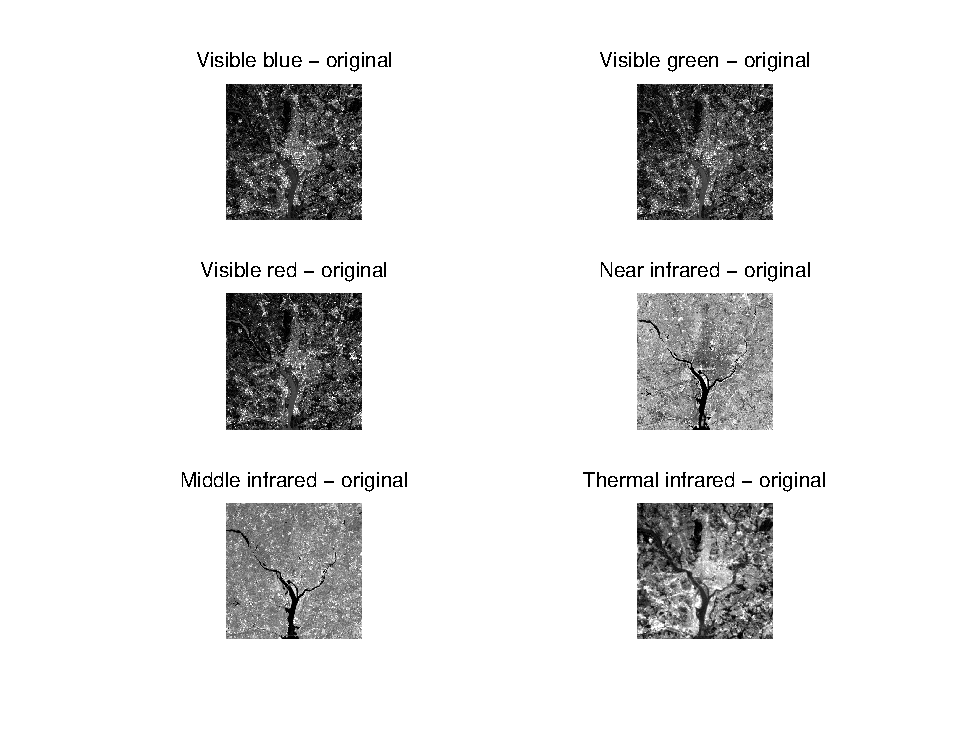
\includegraphics[width=\linewidth]{original_pca.eps}
 \caption{The original images of which the principal image components are computed}
 \label{fig:original_pca}
\end{figure}
\[
\texttt{images} = \begin{bmatrix}
       17  & 22  & \ldots & 26  & 26   \\[0.3em]
       6   & 20  & \ldots & 27  & 27   \\[0.3em]
       9   & 19  & \ldots & 28  & 28   \\[0.3em]
       154 & 98  & \ldots & 149 & 149  \\[0.3em]     
       94  & 101 & \ldots & 116 & 116  \\[0.3em]
       95  & 73  & \ldots & 84  & 84  
\end{bmatrix}
\]
The \texttt{images} does indeed contain 6 rows of the images with \(564^2\) columns.
\clearpage
\subsection{Principal components transform}
\begin{figure}[htb]
 \centering
 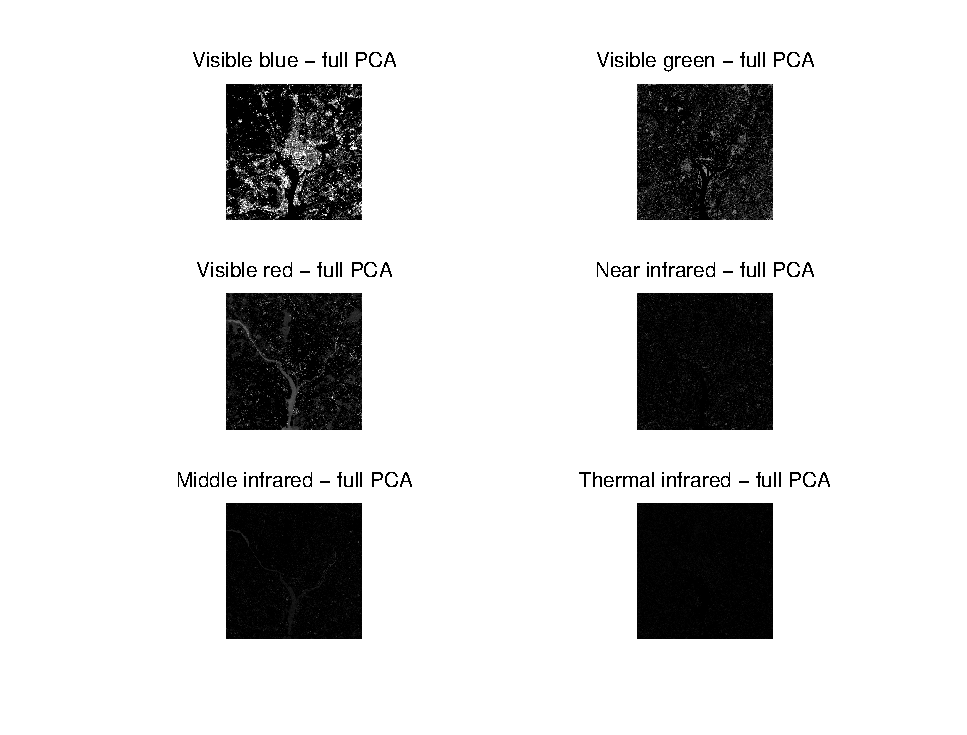
\includegraphics[width=\linewidth]{full_pca.eps}
 \caption{The principal components of the matrix constructed in (b)}
 \label{fig:full_pca}
\end{figure}
Eigenvalues (desc.): 10344, 2966, 1401, 203, 94 and 31.
\clearpage
\subsection{Partial reconstruction}
\begin{figure}[htb]
 \centering
 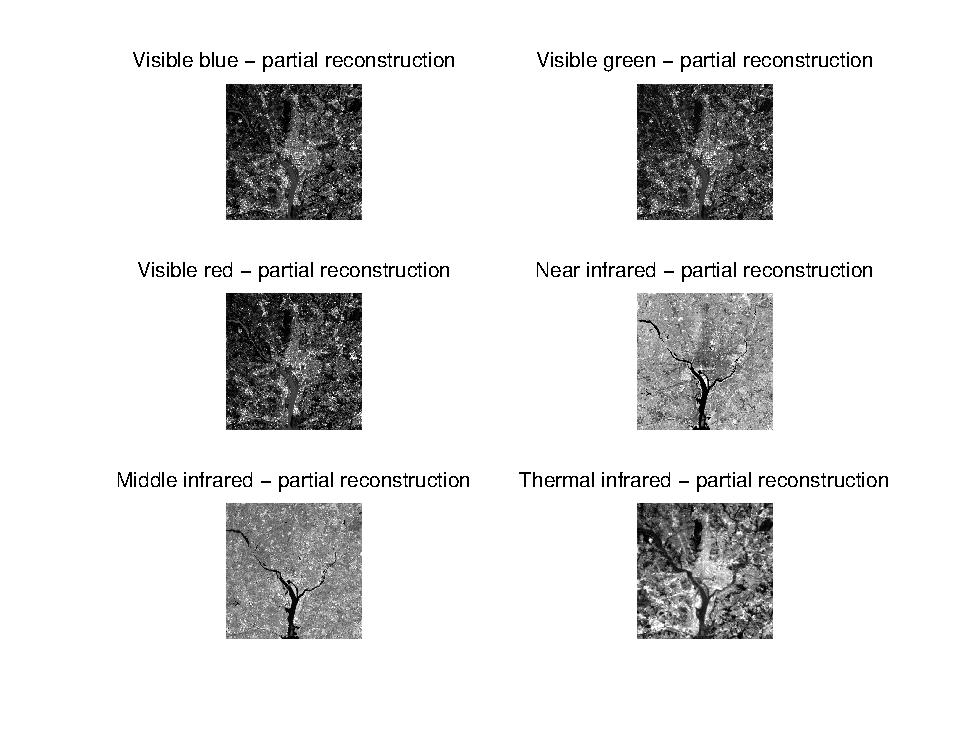
\includegraphics[width=\linewidth]{partial_recon_pca.eps}
 \caption{The reconstruction of the matrix constructed in (b) using three largest eigenvalues}
 \label{fig:partial_recon_pca}
\end{figure}
\begin{figure}[htb]
 \centering
 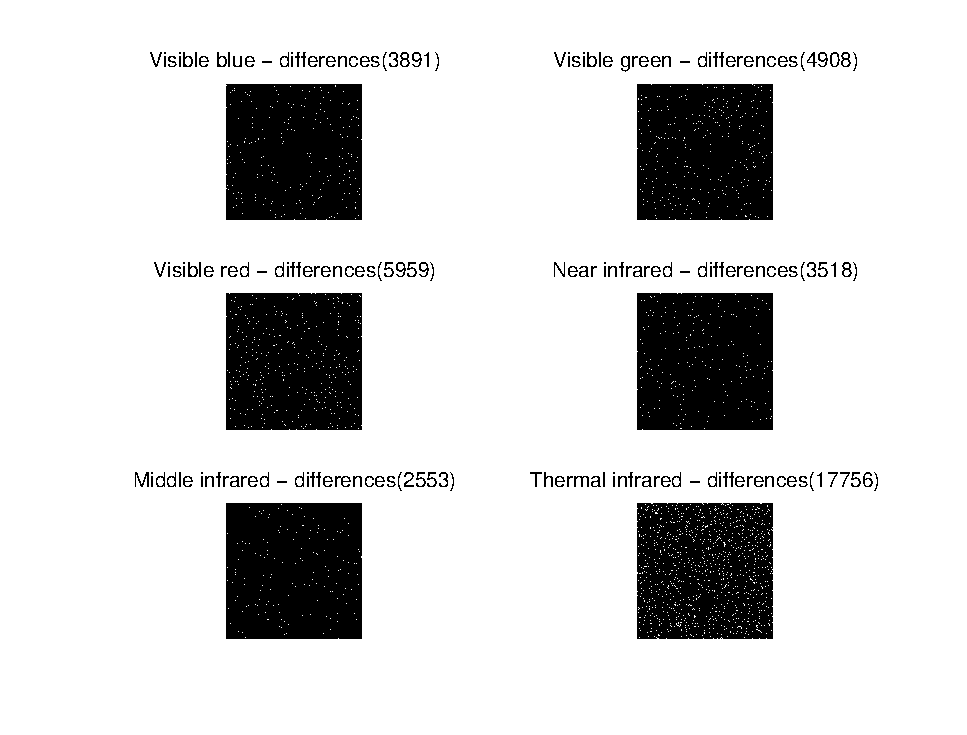
\includegraphics[width=\linewidth]{differences_pca.eps}
 \caption{Difference between the matrix constructed in (b) and the partial reconstruction using three largest eigenvalues}
 \label{fig:differences_pca}
\end{figure}
\clearpage